\documentclass[a4paper,12pt]{article}
\usepackage[utf8]{inputenc}
\usepackage[magyar]{babel}
\usepackage{amsmath, amssymb}
\usepackage{enumitem}
\usepackage{multicol}
\usepackage{graphicx}
\usepackage{wrapfig}
\usepackage[a4paper, margin=25mm]{geometry} % smaller margins
\pagestyle{empty}

\setlength{\parindent}{0pt}
\setlength{\parskip}{10pt}

\begin{document}

Matekórára hozni:
\begin{itemize}
\item Tablet és laptop is, hogy lehessen jól rajzolni
\item Matekfüzet az óráról, kérdések, mit tanultatok?
\item Feladatok ami nem megy vagy nem értetted órán
\item Feladatgyűjtemény
\item Iskolai házifeladat megoldásmenete
\item Gergő+Éva házifeladat megoldásmenete
\end{itemize}

\renewcommand{\arraystretch}{1.5}

%% \begin{enumerate}
%%   \setcounter{enumi}{2}

\begin{wrapfigure}{r}{0.25\textwidth}
  \vspace{-0.5cm}
  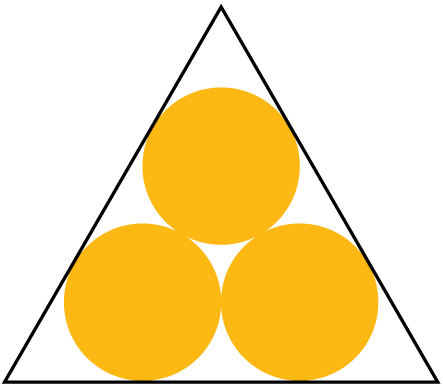
\includegraphics[width=0.25\textwidth]{abra}
\end{wrapfigure}

3) Egy szabályos háromszög alakú ablakkeretet szeretnénk készíteni
három színes ablaküveg köré, melyek mindegyike 30 cm sugarú körlap. A
körökön kívül eső részt átlátszó üvegből készítjük. Hogyan válasszuk
meg a keret oldalainak hosszát, ha azt szeretnénk, hogy az üveg
körlapok (az ábrán látható módon) páronként érintsék egymást, és
mindegyik érintse a keret oldalait is? Válaszod cm-ben, egészekre
kerekítve add meg!

4) Adott három 1 cm sugarú kör úgy, hogy a középpontjaik nincsenek egy
egyenesen. Szerkessz egy kört, amelyik mindhárom adott kört érinti!

\end{document}
